%%%%%%%%%%%%%%%%%%%%%%%%%%%%%%%%%%%%%%%%%%%%%%%%%%%%%%%%%%%%%%%%
\section{实验结果}
%%%%%%%%%%%%%%%%%%%%%%%%%%%%%%%%%%%%%%%%%%%%%%%%%%%%%%%%%%%%%%%%

\subsection{数据说明与描述性统计}

主实验共获得1500条有效观测：5款模型、6种条件、每个模型-条件50次独立无状态API会话。
此外，DeepSeek-V4-Flash和DeepSeek-V4-Pro各增加6个条件下的50次深度思考模式调用，共600条对照观测。
所有返回均成功解析为预定义JSON格式，解析错误率为0\%。
每条记录包含10道Holt-Laury题目的选择序列、理由文本、实验条件、模型名称、思考模式和时间戳。
切换次数检查未发现超过预设阈值的异常记录，因此正式分析未剔除样本。

核心因变量为安全选择数$N_{\text{safe}}$，即10道题中选择较安全选项A的次数。
风险中性基准约为$N_{\text{safe}}=4$；数值越高表示越风险规避，越低表示越风险寻求。
\Cref{tab:descriptive}报告各模型在六种主实验条件下的均值、标准差、中位数和范围。

\begin{table}[tb]
  \caption{各模型在各实验条件下的安全选择数（$N_{\text{safe}}$）描述性统计；各条件样本量均为$n=50$}
  \label{tab:descriptive}
  \centering
  \scriptsize
  \setlength{\tabcolsep}{2.2pt}
  \begin{tabular}{llrrrrr}
    \toprule
    模型 & 条件 & 均值 & $SD$ & 中位数 & 最小值 & 最大值 \\
    \midrule
    \multirow{6}{*}{DeepSeek-V4-Flash} & Gain/Self & 3.92 & 2.41 & 5.0 & 0 & 9 \\
     & Gain/Inv & 4.14 & 2.73 & 5.0 & 0 & 9 \\
     & Gain/Vis & 4.46 & 2.73 & 5.0 & 0 & 9 \\
     & Loss/Self & 4.18 & 2.22 & 4.0 & 0 & 9 \\
     & Loss/Inv & 4.86 & 3.20 & 5.0 & 0 & 10 \\
     & Loss/Vis & 4.58 & 2.37 & 5.0 & 0 & 9 \\
    \multirow{6}{*}{DeepSeek-V4-Pro} & Gain/Self & 3.36 & 1.08 & 3.0 & 0 & 5 \\
     & Gain/Inv & 3.74 & 1.27 & 4.0 & 0 & 9 \\
     & Gain/Vis & 3.74 & 1.16 & 4.0 & 0 & 6 \\
     & Loss/Self & 4.02 & 1.49 & 4.0 & 0 & 10 \\
     & Loss/Inv & 4.36 & 1.68 & 4.0 & 0 & 10 \\
     & Loss/Vis & 3.98 & 1.70 & 4.0 & 0 & 10 \\
    \multirow{6}{*}{Grok-4} & Gain/Self & 4.00 & 0.00 & 4.0 & 4 & 4 \\
     & Gain/Inv & 4.00 & 0.00 & 4.0 & 4 & 4 \\
     & Gain/Vis & 4.00 & 0.00 & 4.0 & 4 & 4 \\
     & Loss/Self & 4.00 & 0.00 & 4.0 & 4 & 4 \\
     & Loss/Inv & 4.00 & 0.00 & 4.0 & 4 & 4 \\
     & Loss/Vis & 4.00 & 0.00 & 4.0 & 4 & 4 \\
    \multirow{6}{*}{Kimi-k2} & Gain/Self & 8.48 & 1.74 & 9.0 & 0 & 9 \\
     & Gain/Inv & 8.14 & 2.11 & 9.0 & 0 & 10 \\
     & Gain/Vis & 8.56 & 1.36 & 9.0 & 4 & 9 \\
     & Loss/Self & 9.38 & 1.24 & 10.0 & 5 & 10 \\
     & Loss/Inv & 9.50 & 1.04 & 10.0 & 5 & 10 \\
     & Loss/Vis & 9.38 & 1.52 & 10.0 & 4 & 10 \\
    \multirow{6}{*}{GPT-4.1} & Gain/Self & 4.92 & 0.27 & 5.0 & 4 & 5 \\
     & Gain/Inv & 4.66 & 0.52 & 5.0 & 3 & 5 \\
     & Gain/Vis & 5.22 & 0.46 & 5.0 & 5 & 7 \\
     & Loss/Self & 6.62 & 1.83 & 5.0 & 5 & 9 \\
     & Loss/Inv & 5.50 & 1.30 & 5.0 & 4 & 9 \\
     & Loss/Vis & 7.28 & 1.78 & 8.0 & 5 & 9 \\
    \bottomrule
  \end{tabular}
\end{table}


\begin{figure}[!htbp]
  \centering
  \tikzset{
  every picture/.style={font=\scriptsize},
}
\definecolor{dsflash}{HTML}{4E79A7}
\definecolor{dspro}{HTML}{F28E2B}
\definecolor{grokc}{HTML}{59A14F}
\definecolor{kimic}{HTML}{E15759}
\definecolor{gptc}{HTML}{B07AA1}
\definecolor{gridgray}{HTML}{D9D9D9}
\definecolor{riskred}{HTML}{B2182B}
\definecolor{riskorange}{HTML}{EF8A62}
\definecolor{riskorangeone}{HTML}{FDAE61}
\definecolor{riskyellow}{HTML}{FDDC8B}
\definecolor{riskneutral}{HTML}{FFFFBF}
\definecolor{riskgreenone}{HTML}{D9EF8B}
\definecolor{riskgreentwo}{HTML}{A6D96A}
\definecolor{riskgreenthree}{HTML}{66BD63}
\definecolor{riskgreenfour}{HTML}{1A9850}

\begin{tikzpicture}
\begin{axis}[
  width=\linewidth,
  height=0.25\textheight,
  ybar,
  ymin=0,
  ymax=10.5,
  ylabel={$N_{\mathrm{safe}}$},
  symbolic x coords={G/Self,G/Inv,G/Vis,L/Self,L/Inv,L/Vis},
  xtick=data,
  enlarge x limits=0.10,
  xticklabel style={font=\tiny, rotate=35, anchor=east},
  tick label style={font=\tiny},
  label style={font=\scriptsize},
  legend style={font=\tiny, draw=none, fill=none, at={(0.5,1.05)}, anchor=south, legend columns=3},
  ymajorgrids=true,
  grid style={gridgray},
]
\addplot[ybar, bar width=2.4pt, fill=dsflash, draw=none] coordinates {(G/Self,3.920) (G/Inv,4.140) (G/Vis,4.460) (L/Self,4.180) (L/Inv,4.860) (L/Vis,4.580)};
\addplot[ybar, bar width=2.4pt, fill=dspro, draw=none] coordinates {(G/Self,3.360) (G/Inv,3.740) (G/Vis,3.740) (L/Self,4.020) (L/Inv,4.360) (L/Vis,3.980)};
\addplot[ybar, bar width=2.4pt, fill=grokc, draw=none] coordinates {(G/Self,4.000) (G/Inv,4.000) (G/Vis,4.000) (L/Self,4.000) (L/Inv,4.000) (L/Vis,4.000)};
\addplot[ybar, bar width=2.4pt, fill=kimic, draw=none] coordinates {(G/Self,8.480) (G/Inv,8.140) (G/Vis,8.560) (L/Self,9.380) (L/Inv,9.500) (L/Vis,9.380)};
\addplot[ybar, bar width=2.4pt, fill=gptc, draw=none] coordinates {(G/Self,4.920) (G/Inv,4.660) (G/Vis,5.220) (L/Self,6.620) (L/Inv,5.500) (L/Vis,7.280)};
\addplot[black, dashed, sharp plot, forget plot] coordinates {(G/Self,4) (L/Vis,4)};
\legend{DeepSeek-V4-Flash,DeepSeek-V4-Pro,Grok-4,Kimi-k2,GPT-4.1}
\end{axis}
\end{tikzpicture}

  \caption{五款模型在六种实验条件下的平均安全选择数。虚线表示风险中性基准$N_{\text{safe}}=4$。}
  \label{fig:mean_comparison}
\end{figure}

描述性结果已经显示出强烈模型异质性。
Grok-4在整卷作答中始终给出$N_{\text{safe}}=4$，表现为风险中性且方差为0；Kimi-k2在所有条件下均远高于中性线，尤其在损失域接近量表上限；GPT-4.1和DeepSeek V4系列则更受条件变化影响。
因此，后续假设检验均在模型内报告，并统一同时给出原始$p$值和Benjamini-Hochberg校正后的$q_{BH}$。
这种呈现方式有两个考虑。
首先，若直接将五款模型混合比较，模型身份本身会吞没角色和问责性操纵的影响，使H1和H2难以解释。
其次，LLM重复调用并不等同于人类随机抽样，被试间方差更多反映同一模型在给定Prompt下的生成分布。
因此，本文更重视模型内条件变化、校正后的显著性以及效应方向是否与理论假设一致，而不是仅依赖总体均值差异。

\subsection{假设检验}

\subsubsection{H1A/H1B：代理角色效应}

H1A和H1B主要针对收益域内的代理偏移提出。
\Cref{tab:gain_agent_effect}显示，收益域中DeepSeek-V4-Pro和DeepSeek-V4-Flash虽呈谨慎化方向，但校正后均不显著。
GPT-4.1呈现最清晰但方向相反的条件性效应：不可观察代理条件低于Self条件（风险放松，$q_{BH}=0.019$），可观察代理条件高于Self条件（谨慎化，$q_{BH}<0.001$）。
这意味着“替他人决策”本身并不对应单一方向，至少在GPT-4.1中必须同时考虑可观察性。

\begin{table*}[tb]
  \caption{收益域代理角色效应检验（置换检验，双侧；各条件$n=50$）}
  \label{tab:gain_agent_effect}
  \centering
  \scriptsize
  \setlength{\tabcolsep}{3.2pt}
  \begin{tabular}{lrrrrrrrrr}
    \toprule
    模型 & Self均值 & Inv均值 & Vis均值 & $\Delta_{Inv-Self}$ & $p$ & $q_{BH}$ & $\Delta_{Vis-Self}$ & $p$ & $q_{BH}$ \\
    \midrule
    DeepSeek-V4-Flash & 3.92 & 4.14 & 4.46 & +0.22 & 0.698 & 0.997 & +0.54 & 0.314 & 0.628 \\
    DeepSeek-V4-Pro & 3.36 & 3.74 & 3.74 & +0.38 & 0.134 & 0.334 & +0.38 & 0.112 & 0.334 \\
    Grok-4 & 4.00 & 4.00 & 4.00 & +0.00 & 1.000 & 1.000 & +0.00 & 1.000 & 1.000 \\
    Kimi-k2 & 8.48 & 8.14 & 8.56 & -0.34 & 0.420 & 0.699 & +0.08 & 0.842 & 1.000 \\
    GPT-4.1 & 4.92 & 4.66 & 5.22 & -0.26 & 0.004 & \textbf{0.019} & +0.30 & $<0.001$ & \textbf{$<0.001$} \\
    \bottomrule
  \end{tabular}
  \vspace{0.25em}

  \parbox{0.96\textwidth}{\footnotesize 注：$\Delta>0$表示相对于Self条件更谨慎，$\Delta<0$表示更冒险。置换检验以$N_{\text{safe}}$均值差为统计量，迭代20,000次，随机种子固定；$q_{BH}$为本表10个成对检验的Benjamini-Hochberg校正值。}
\end{table*}


作为补充，我们将收益域与损失域合并，比较Self条件与全部Agent条件。
\Cref{tab:agent_effect}显示，校正后仅DeepSeek-V4-Pro存在轻度总体谨慎偏移（$q_{BH}=0.035$）。
由于该检验跨越损益域，它只能作为代理角色总体效应的补充证据，不能替代收益域内的H1主检验。

\begin{table*}[tb]
  \caption{代理角色主效应检验结果（Mann-Whitney U检验）}
  \label{tab:agent_effect}
  \centering
  \footnotesize
  \setlength{\tabcolsep}{4pt}
  \begin{tabular}{lrrlrrrl}
    \toprule
    模型 & Self均值 & Agent均值 & 偏移方向 & $U$统计量 & $p$ & $q_{BH}$ & 效应判定 \\
    \midrule
    DeepSeek-V4-Flash & 4.05 & 4.51 & +0.46（谨慎$\uparrow$） & 8911.0 & 0.115 & 0.288 & 不显著 \\
    DeepSeek-V4-Pro & 3.69 & 3.96 & +0.27（谨慎$\uparrow$） & 8222.0 & \textbf{0.007} & \textbf{0.035} & \textbf{显著} \\
    Grok-4 & 4.00 & 4.00 & 0.00 & -- & 1.000 & 1.000 & 无效应 \\
    Kimi-k2 & 8.93 & 8.89 & -0.04 & 9893.5 & 0.867 & 1.000 & 不显著 \\
    GPT-4.1 & 5.77 & 5.67 & -0.10 & 10219.0 & 0.711 & 1.000 & 不显著 \\
    \bottomrule
  \end{tabular}
  \vspace{0.25em}

  \parbox{0.96\textwidth}{\footnotesize 注：$q_{BH}$为本表5个模型检验的Benjamini-Hochberg校正值。}
\end{table*}


\subsubsection{H2：问责性与损益域的调节}

问责性检验首先比较Self、Agent-Invisible和Agent-Visible三类角色条件。
\Cref{tab:accountability_effect}显示，GPT-4.1在三类条件之间差异显著（$q_{BH}=0.005$）；DeepSeek-V4-Pro虽有原始$p=0.027$，但BH校正后$q_{BH}=0.068$，因此仅能视为趋势。
这一步说明问责性效应并非跨模型普遍存在。

\begin{table}[tb]
  \caption{问责性调节效应检验结果（Kruskal-Wallis H检验）}
  \label{tab:accountability_effect}
  \centering
  \footnotesize
  \setlength{\tabcolsep}{2.2pt}
  \resizebox{\linewidth}{!}{%
  \begin{tabular}{lrrrrrr}
    \toprule
    模型 & Self均值 & Agent-Inv均值 & Agent-Vis均值 & $H$ & $p$ & $q_{BH}$ \\
    \midrule
    DeepSeek-V4-Flash & 4.05 & 4.50 & 4.52 & 2.57 & 0.277 & 0.462 \\
    DeepSeek-V4-Pro & 3.69 & 4.05 & 3.86 & 7.25 & 0.027 & 0.068 \\
    Grok-4 & 4.00 & 4.00 & 4.00 & 0.00 & 1.000 & 1.000 \\
    Kimi-k2 & 8.93 & 8.82 & 8.97 & 0.60 & 0.743 & 0.929 \\
    GPT-4.1 & 5.77 & 5.08 & 6.25 & 45.73 & \textbf{$<0.001$} & \textbf{0.005} \\
    \bottomrule
  \end{tabular}}
  \vspace{0.25em}

  \parbox{0.96\linewidth}{\footnotesize 注：$q_{BH}$为本表5个模型检验的Benjamini-Hochberg校正值。}
\end{table}


为直接检验H2所要求的损益域$\times$问责性模式，我们在Agent条件内部计算差中差（$L/G$分别表示损失域/收益域，$V/I$分别表示可观察/不可观察）：
\[
  \begin{aligned}
  \text{DiD}
  =(\bar N_{L,V}-\bar N_{L,I})
  -(\bar N_{G,V}-\bar N_{G,I}).
  \end{aligned}
\]
\Cref{tab:domain_accountability_interaction}显示，仅GPT-4.1在BH校正后仍显著（DiD=+1.22，$q_{BH}=0.025$）。
也就是说，可见性带来的谨慎化在GPT-4.1的损失域中更强；其他模型未呈现同样模式。

\begin{table}[tb]
  \caption{问责可见性与损益域的差中差检验（Agent条件内置换检验）}
  \label{tab:domain_accountability_interaction}
  \centering
  \scriptsize
  \setlength{\tabcolsep}{3.5pt}
  \begin{tabular}{lrrrrr}
    \toprule
    模型 & $\Delta^{Gain}_{Vis-Inv}$ & $\Delta^{Loss}_{Vis-Inv}$ & DiD & $p$ & $q_{BH}$ \\
    \midrule
    DeepSeek-V4-Flash & +0.32 & -0.28 & -0.60 & 0.458 & 0.573 \\
    DeepSeek-V4-Pro & +0.00 & -0.38 & -0.38 & 0.399 & 0.573 \\
    Grok-4 & +0.00 & +0.00 & +0.00 & 1.000 & 1.000 \\
    Kimi-k2 & +0.42 & -0.12 & -0.54 & 0.266 & 0.573 \\
    GPT-4.1 & +0.56 & +1.78 & +1.22 & 0.005 & \textbf{0.025} \\
    \bottomrule
  \end{tabular}
  \vspace{0.25em}

  \parbox{0.96\linewidth}{\footnotesize 注：DiD=$\Delta^{Loss}_{Vis-Inv}-\Delta^{Gain}_{Vis-Inv}$。正值表示可见性带来的谨慎化在损失域更强。检验仅使用Agent-Invisible与Agent-Visible条件，置换检验迭代20,000次；$q_{BH}$为本表5个模型检验的Benjamini-Hochberg校正值。}
\end{table}


\begin{figure}[!htbp]
  \centering
  \makebox[\linewidth][c]{\hspace*{-0.140\linewidth}\resizebox{0.92\linewidth}{!}{\tikzset{
  every picture/.style={font=\scriptsize},
}
\definecolor{dsflash}{HTML}{4E79A7}
\definecolor{dspro}{HTML}{F28E2B}
\definecolor{grokc}{HTML}{59A14F}
\definecolor{kimic}{HTML}{E15759}
\definecolor{gptc}{HTML}{B07AA1}
\definecolor{gridgray}{HTML}{D9D9D9}
\definecolor{riskred}{HTML}{B2182B}
\definecolor{riskorange}{HTML}{EF8A62}
\definecolor{riskorangeone}{HTML}{FDAE61}
\definecolor{riskyellow}{HTML}{FDDC8B}
\definecolor{riskneutral}{HTML}{FFFFBF}
\definecolor{riskgreenone}{HTML}{D9EF8B}
\definecolor{riskgreentwo}{HTML}{A6D96A}
\definecolor{riskgreenthree}{HTML}{66BD63}
\definecolor{riskgreenfour}{HTML}{1A9850}

\begin{tikzpicture}
\begin{axis}[
  width=\linewidth,
  height=0.27\textheight,
  tick label style={font=\tiny},
  label style={font=\scriptsize},
  legend style={font=\tiny, draw=none, fill=none},
  ymajorgrids=true,
  grid style={gridgray},
  ymin=0,
  ymax=10.5,
  ylabel={$N_{\mathrm{safe}}$},
  height=0.215\textheight, symbolic x coords={Gain,Loss}, xtick=data, legend pos=north west, xlabel={domain},
]
\addplot+[mark=*, thick, gptc] coordinates {(Gain,4.920) (Loss,6.620)};
\addplot+[mark=*, thick, dsflash] coordinates {(Gain,4.660) (Loss,5.500)};
\addplot+[mark=*, thick, grokc] coordinates {(Gain,5.220) (Loss,7.280)};
\addplot+[black, dashed, sharp plot, forget plot] coordinates {(Gain,4) (Loss,4)};
\legend{Self,Invisible,Visible}
\end{axis}
\end{tikzpicture}
}}
  \caption{GPT-4.1中损益域与问责性的分化模式。}
  \label{fig:gpt_interaction}
\end{figure}

\subsubsection{损益域框架效应}

传统前景理论预测人类在损失域更可能风险寻求。
但\Cref{tab:domain_effect}显示，DeepSeek-V4-Pro、Kimi-k2和GPT-4.1在损失域的$N_{\text{safe}}$均显著高于收益域，且BH校正后仍成立。
这构成了本研究的“反前景理论”现象：多数模型面对损失语义时不是更冒险，而是更防御、更保守。

\begin{table}[tb]
  \caption{损益域框架效应检验结果}
  \label{tab:domain_effect}
  \centering
  \footnotesize
  \setlength{\tabcolsep}{3pt}
  \resizebox{\linewidth}{!}{%
  \begin{tabular}{lrrlrrr}
    \toprule
    模型 & 收益域 & 损失域 & 偏移方向 & $U$ & $p$ & $q_{BH}$ \\
    \midrule
    DeepSeek-V4-Flash & 4.17 & 4.54 & +0.37 & 10755.0 & 0.499 & 0.624 \\
    DeepSeek-V4-Pro & 3.61 & 4.12 & +0.51 & 8936.5 & \textbf{0.001} & \textbf{0.002} \\
    Grok-4 & 4.00 & 4.00 & 0.00 & -- & 1.000 & 1.000 \\
    Kimi-k2 & 8.39 & 9.42 & +1.03 & 3794.5 & \textbf{$<0.001$} & \textbf{0.002} \\
    GPT-4.1 & 4.93 & 6.47 & +1.54 & 5927.0 & \textbf{$<0.001$} & \textbf{0.002} \\
    \bottomrule
  \end{tabular}}
  \vspace{0.25em}

  \parbox{0.96\linewidth}{\footnotesize 注：$q_{BH}$为本表5个模型检验的Benjamini-Hochberg校正值。}
\end{table}


\begin{figure}[!ht]
  \centering
  \begin{minipage}{\linewidth}
    \centering
    \makebox[\linewidth][c]{\hspace*{-0.130\linewidth}\resizebox{0.98\linewidth}{!}{\tikzset{
  every picture/.style={font=\scriptsize},
}
\definecolor{dsflash}{HTML}{4E79A7}
\definecolor{dspro}{HTML}{F28E2B}
\definecolor{grokc}{HTML}{59A14F}
\definecolor{kimic}{HTML}{E15759}
\definecolor{gptc}{HTML}{B07AA1}
\definecolor{gridgray}{HTML}{D9D9D9}
\definecolor{riskred}{HTML}{B2182B}
\definecolor{riskorange}{HTML}{EF8A62}
\definecolor{riskorangeone}{HTML}{FDAE61}
\definecolor{riskyellow}{HTML}{FDDC8B}
\definecolor{riskneutral}{HTML}{FFFFBF}
\definecolor{riskgreenone}{HTML}{D9EF8B}
\definecolor{riskgreentwo}{HTML}{A6D96A}
\definecolor{riskgreenthree}{HTML}{66BD63}
\definecolor{riskgreenfour}{HTML}{1A9850}

\begin{tikzpicture}
\begin{groupplot}[
  group style={group name=g, group size=3 by 2, horizontal sep=0.48cm, vertical sep=0.62cm},
  width=0.33\linewidth,
  height=0.36\textheight/2.35,
  tick label style={font=\tiny},
  label style={font=\tiny},
  title style={font=\tiny},
  ymajorgrids=true,
  grid style={gridgray},
]
\nextgroupplot[
  title={G/Self},
  ymin=0,
  ymax=54.3,
  xmin=-0.5,
  xmax=10.5,
  xtick={0,2,4,6,8,10},
  yticklabel style={font=\tiny},
  xticklabels={},
  ylabel={freq},
]
\addplot[ybar, bar width=4.6pt, fill=gptc, draw=none] coordinates {(0,0.000) (1,0.000) (2,0.000) (3,0.000) (4,4.000) (5,46.000) (6,0.000) (7,0.000) (8,0.000) (9,0.000) (10,0.000)};
\addplot[red, dashed, thick, forget plot] coordinates {(4.92,0) (4.92,48.3)};
\node[anchor=north east, font=\tiny, fill=white, fill opacity=0.78, text opacity=1, inner sep=1pt] at (rel axis cs:0.98,0.98) {Mean=4.92};
\nextgroupplot[
  title={G/Inv},
  ymin=0,
  ymax=40.1,
  xmin=-0.5,
  xmax=10.5,
  xtick={0,2,4,6,8,10},
  yticklabel style={font=\tiny},
  xticklabels={},
]
\addplot[ybar, bar width=4.6pt, fill=gptc, draw=none] coordinates {(0,0.000) (1,0.000) (2,0.000) (3,1.000) (4,15.000) (5,34.000) (6,0.000) (7,0.000) (8,0.000) (9,0.000) (10,0.000)};
\addplot[red, dashed, thick, forget plot] coordinates {(4.66,0) (4.66,35.7)};
\node[anchor=north east, font=\tiny, fill=white, fill opacity=0.78, text opacity=1, inner sep=1pt] at (rel axis cs:0.98,0.98) {Mean=4.66};
\nextgroupplot[
  title={G/Vis},
  ymin=0,
  ymax=47.2,
  xmin=-0.5,
  xmax=10.5,
  xtick={0,2,4,6,8,10},
  yticklabel style={font=\tiny},
  xticklabels={},
]
\addplot[ybar, bar width=4.6pt, fill=gptc, draw=none] coordinates {(0,0.000) (1,0.000) (2,0.000) (3,0.000) (4,0.000) (5,40.000) (6,9.000) (7,1.000) (8,0.000) (9,0.000) (10,0.000)};
\addplot[red, dashed, thick, forget plot] coordinates {(5.22,0) (5.22,42.0)};
\node[anchor=north east, font=\tiny, fill=white, fill opacity=0.78, text opacity=1, inner sep=1pt] at (rel axis cs:0.98,0.98) {Mean=5.22};
\nextgroupplot[
  title={L/Self},
  ymin=0,
  ymax=30.7,
  xmin=-0.5,
  xmax=10.5,
  xtick={0,2,4,6,8,10},
  yticklabel style={font=\tiny},
  xlabel={$N_{\mathrm{safe}}$},
  ylabel={freq},
]
\addplot[ybar, bar width=4.6pt, fill=gptc, draw=none] coordinates {(0,0.000) (1,0.000) (2,0.000) (3,0.000) (4,0.000) (5,26.000) (6,2.000) (7,2.000) (8,5.000) (9,15.000) (10,0.000)};
\addplot[red, dashed, thick, forget plot] coordinates {(6.62,0) (6.62,27.3)};
\node[anchor=north east, font=\tiny, fill=white, fill opacity=0.78, text opacity=1, inner sep=1pt] at (rel axis cs:0.98,0.98) {Mean=6.62};
\nextgroupplot[
  title={L/Inv},
  ymin=0,
  ymax=48.4,
  xmin=-0.5,
  xmax=10.5,
  xtick={0,2,4,6,8,10},
  yticklabel style={font=\tiny},
  xlabel={$N_{\mathrm{safe}}$},
]
\addplot[ybar, bar width=4.6pt, fill=gptc, draw=none] coordinates {(0,0.000) (1,0.000) (2,0.000) (3,0.000) (4,1.000) (5,41.000) (6,1.000) (7,1.000) (8,1.000) (9,5.000) (10,0.000)};
\addplot[red, dashed, thick, forget plot] coordinates {(5.50,0) (5.50,43.1)};
\node[anchor=north east, font=\tiny, fill=white, fill opacity=0.78, text opacity=1, inner sep=1pt] at (rel axis cs:0.98,0.98) {Mean=5.50};
\nextgroupplot[
  title={L/Vis},
  ymin=0,
  ymax=27.1,
  xmin=-0.5,
  xmax=10.5,
  xtick={0,2,4,6,8,10},
  yticklabel style={font=\tiny},
  xlabel={$N_{\mathrm{safe}}$},
]
\addplot[ybar, bar width=4.6pt, fill=gptc, draw=none] coordinates {(0,0.000) (1,0.000) (2,0.000) (3,0.000) (4,0.000) (5,15.000) (6,5.000) (7,4.000) (8,3.000) (9,23.000) (10,0.000)};
\addplot[red, dashed, thick, forget plot] coordinates {(7.28,0) (7.28,24.2)};
\node[anchor=north east, font=\tiny, fill=white, fill opacity=0.78, text opacity=1, inner sep=1pt] at (rel axis cs:0.98,0.98) {Mean=7.28};
\end{groupplot}
\end{tikzpicture}
}}
    \subcaption{GPT-4.1各条件下$N_{\text{safe}}$分布。}
    \label{fig:gpt_distribution}
  \end{minipage}
  \vspace{0.1em}

  \begin{minipage}{\linewidth}
    \centering
    \makebox[\linewidth][c]{\hspace*{-0.130\linewidth}\resizebox{0.98\linewidth}{!}{\tikzset{
  every picture/.style={font=\scriptsize},
}
\definecolor{dsflash}{HTML}{4E79A7}
\definecolor{dspro}{HTML}{F28E2B}
\definecolor{grokc}{HTML}{59A14F}
\definecolor{kimic}{HTML}{E15759}
\definecolor{gptc}{HTML}{B07AA1}
\definecolor{gridgray}{HTML}{D9D9D9}
\definecolor{riskred}{HTML}{B2182B}
\definecolor{riskorange}{HTML}{EF8A62}
\definecolor{riskorangeone}{HTML}{FDAE61}
\definecolor{riskyellow}{HTML}{FDDC8B}
\definecolor{riskneutral}{HTML}{FFFFBF}
\definecolor{riskgreenone}{HTML}{D9EF8B}
\definecolor{riskgreentwo}{HTML}{A6D96A}
\definecolor{riskgreenthree}{HTML}{66BD63}
\definecolor{riskgreenfour}{HTML}{1A9850}

\begin{tikzpicture}
\begin{groupplot}[
  group style={group name=g, group size=3 by 2, horizontal sep=0.48cm, vertical sep=0.62cm},
  width=0.33\linewidth,
  height=0.36\textheight/2.35,
  tick label style={font=\tiny},
  label style={font=\tiny},
  title style={font=\tiny},
  ymajorgrids=true,
  grid style={gridgray},
]
\nextgroupplot[
  title={G/Self},
  ymin=0,
  ymax=53.1,
  xmin=-0.5,
  xmax=10.5,
  xtick={0,2,4,6,8,10},
  yticklabel style={font=\tiny},
  xticklabels={},
  ylabel={freq},
]
\addplot[ybar, bar width=4.6pt, fill=kimic, draw=none] coordinates {(0,1.000) (1,0.000) (2,0.000) (3,1.000) (4,1.000) (5,1.000) (6,0.000) (7,1.000) (8,0.000) (9,45.000) (10,0.000)};
\addplot[red, dashed, thick, forget plot] coordinates {(8.48,0) (8.48,47.2)};
\node[anchor=north east, font=\tiny, fill=white, fill opacity=0.78, text opacity=1, inner sep=1pt] at (rel axis cs:0.98,0.98) {Mean=8.48};
\nextgroupplot[
  title={G/Inv},
  ymin=0,
  ymax=46.0,
  xmin=-0.5,
  xmax=10.5,
  xtick={0,2,4,6,8,10},
  yticklabel style={font=\tiny},
  xticklabels={},
]
\addplot[ybar, bar width=4.6pt, fill=kimic, draw=none] coordinates {(0,2.000) (1,0.000) (2,0.000) (3,0.000) (4,0.000) (5,4.000) (6,3.000) (7,0.000) (8,1.000) (9,39.000) (10,1.000)};
\addplot[red, dashed, thick, forget plot] coordinates {(8.14,0) (8.14,41.0)};
\node[anchor=north east, font=\tiny, fill=white, fill opacity=0.78, text opacity=1, inner sep=1pt] at (rel axis cs:0.98,0.98) {Mean=8.14};
\nextgroupplot[
  title={G/Vis},
  ymin=0,
  ymax=53.1,
  xmin=-0.5,
  xmax=10.5,
  xtick={0,2,4,6,8,10},
  yticklabel style={font=\tiny},
  xticklabels={},
]
\addplot[ybar, bar width=4.6pt, fill=kimic, draw=none] coordinates {(0,0.000) (1,0.000) (2,0.000) (3,0.000) (4,3.000) (5,1.000) (6,1.000) (7,0.000) (8,0.000) (9,45.000) (10,0.000)};
\addplot[red, dashed, thick, forget plot] coordinates {(8.56,0) (8.56,47.2)};
\node[anchor=north east, font=\tiny, fill=white, fill opacity=0.78, text opacity=1, inner sep=1pt] at (rel axis cs:0.98,0.98) {Mean=8.56};
\nextgroupplot[
  title={L/Self},
  ymin=0,
  ymax=41.3,
  xmin=-0.5,
  xmax=10.5,
  xtick={0,2,4,6,8,10},
  yticklabel style={font=\tiny},
  xlabel={$N_{\mathrm{safe}}$},
  ylabel={freq},
]
\addplot[ybar, bar width=4.6pt, fill=kimic, draw=none] coordinates {(0,0.000) (1,0.000) (2,0.000) (3,0.000) (4,0.000) (5,1.000) (6,3.000) (7,1.000) (8,1.000) (9,9.000) (10,35.000)};
\addplot[red, dashed, thick, forget plot] coordinates {(9.38,0) (9.38,36.8)};
\node[anchor=north east, font=\tiny, fill=white, fill opacity=0.78, text opacity=1, inner sep=1pt] at (rel axis cs:0.98,0.98) {Mean=9.38};
\nextgroupplot[
  title={L/Inv},
  ymin=0,
  ymax=38.9,
  xmin=-0.5,
  xmax=10.5,
  xtick={0,2,4,6,8,10},
  yticklabel style={font=\tiny},
  xlabel={$N_{\mathrm{safe}}$},
]
\addplot[ybar, bar width=4.6pt, fill=kimic, draw=none] coordinates {(0,0.000) (1,0.000) (2,0.000) (3,0.000) (4,0.000) (5,2.000) (6,0.000) (7,0.000) (8,0.000) (9,15.000) (10,33.000)};
\addplot[red, dashed, thick, forget plot] coordinates {(9.50,0) (9.50,34.6)};
\node[anchor=north east, font=\tiny, fill=white, fill opacity=0.78, text opacity=1, inner sep=1pt] at (rel axis cs:0.98,0.98) {Mean=9.50};
\nextgroupplot[
  title={L/Vis},
  ymin=0,
  ymax=46.0,
  xmin=-0.5,
  xmax=10.5,
  xtick={0,2,4,6,8,10},
  yticklabel style={font=\tiny},
  xlabel={$N_{\mathrm{safe}}$},
]
\addplot[ybar, bar width=4.6pt, fill=kimic, draw=none] coordinates {(0,0.000) (1,0.000) (2,0.000) (3,0.000) (4,1.000) (5,3.000) (6,1.000) (7,0.000) (8,0.000) (9,6.000) (10,39.000)};
\addplot[red, dashed, thick, forget plot] coordinates {(9.38,0) (9.38,41.0)};
\node[anchor=north east, font=\tiny, fill=white, fill opacity=0.78, text opacity=1, inner sep=1pt] at (rel axis cs:0.98,0.98) {Mean=9.38};
\end{groupplot}
\end{tikzpicture}
}}
    \subcaption{Kimi-k2各条件下$N_{\text{safe}}$分布。}
    \label{fig:kimi_distribution}
  \end{minipage}
  \caption{GPT-4.1与Kimi-k2在六种实验条件下的安全选择数分布直方图。}
  \label{fig:domain_distributions}
\end{figure}

\subsubsection{H3：模型间异质性}

跨五款模型的Kruskal-Wallis检验显示，模型身份对$N_{\text{safe}}$具有很强解释力（$H=857.09,p=3.30\times10^{-184}$）。
结合均值与分布，可以概括出三种行为轮廓：Grok-4在整卷作答中近似风险中性；Kimi-k2呈极度保守和天花板效应；GPT-4.1与DeepSeek V4系列更具情境敏感性。
因此，H3获得支持，但其含义不是“所有LLM都有同一种风险偏好”，而是相反：风险偏好必须按模型、任务格式和提示语境分别审计。

\subsection{附加与稳健性分析}

\subsubsection{深度思考模式}

DeepSeek V4系列的深度思考对照显示，开启thinking后两款模型的$N_{\text{safe}}$均向风险中性点收敛，BH校正后仍显著。
这提示部分风险偏差可能来自快速语义响应；当模型显式计算期望值时，社会性线索和损失语义的影响会被削弱。

\begin{table}[tb]
  \caption{DeepSeek V4深度思考模式对比检验}
  \label{tab:thinking_effect}
  \centering
  \footnotesize
  \setlength{\tabcolsep}{3pt}
  \resizebox{\linewidth}{!}{%
  \begin{tabular}{lrrrrrr}
    \toprule
    模型 & Disabled均值 & Enabled均值 & $\Delta$ & $U$ & $p$ & $q_{BH}$ \\
    \midrule
    DeepSeek-V4-Flash & 4.36 & 4.01 & -0.35 & 33001.5 & \textbf{$<0.001$} & \textbf{0.002} \\
    DeepSeek-V4-Pro & 3.87 & 4.03 & +0.16 & 49779.0 & \textbf{0.004} & \textbf{0.004} \\
    \bottomrule
  \end{tabular}}
\end{table}


\begin{figure}[!htbp]
  \centering
  \tikzset{
  every picture/.style={font=\scriptsize},
}
\definecolor{dsflash}{HTML}{4E79A7}
\definecolor{dspro}{HTML}{F28E2B}
\definecolor{grokc}{HTML}{59A14F}
\definecolor{kimic}{HTML}{E15759}
\definecolor{gptc}{HTML}{B07AA1}
\definecolor{gridgray}{HTML}{D9D9D9}
\definecolor{riskred}{HTML}{B2182B}
\definecolor{riskorange}{HTML}{EF8A62}
\definecolor{riskorangeone}{HTML}{FDAE61}
\definecolor{riskyellow}{HTML}{FDDC8B}
\definecolor{riskneutral}{HTML}{FFFFBF}
\definecolor{riskgreenone}{HTML}{D9EF8B}
\definecolor{riskgreentwo}{HTML}{A6D96A}
\definecolor{riskgreenthree}{HTML}{66BD63}
\definecolor{riskgreenfour}{HTML}{1A9850}

\begin{tikzpicture}
\begin{axis}[
  width=\linewidth,
  height=0.27\textheight,
  tick label style={font=\tiny},
  label style={font=\scriptsize},
  legend style={font=\tiny, draw=none, fill=none},
  ymajorgrids=true,
  grid style={gridgray},
  ymin=0,
  ymax=10.5,
  ylabel={$N_{\mathrm{safe}}$},
  width=0.58\linewidth, height=0.19\textheight, ybar, symbolic x coords={DeepSeek-V4-Flash,DeepSeek-V4-Pro}, xtick=data, xticklabel style={font=\tiny}, enlarge x limits=0.34, legend style={font=\tiny, draw=none, fill=white, fill opacity=0.9, text opacity=1, at={(0.98,0.98)}, anchor=north east},
]
\addplot[ybar, bar width=14pt, bar shift=-8pt, fill=dsflash, draw=none, error bars/.cd, y dir=both, y explicit, error bar style={black, thick}] coordinates {(DeepSeek-V4-Flash,4.357) +- (0,0.152) (DeepSeek-V4-Pro,3.867) +- (0,0.083)};
\addplot[ybar, bar width=14pt, bar shift=8pt, fill=dspro, draw=none, error bars/.cd, y dir=both, y explicit, error bar style={black, thick}] coordinates {(DeepSeek-V4-Flash,4.013) +- (0,0.013) (DeepSeek-V4-Pro,4.030) +- (0,0.012)};
\addplot[black, dashed, sharp plot, forget plot] coordinates {(DeepSeek-V4-Flash,4) (DeepSeek-V4-Pro,4)};
\legend{disabled, enabled}
\end{axis}
\end{tikzpicture}

  \caption{DeepSeek V4系列模型在关闭与开启深度思考模式下的安全选择数对比。}
  \label{fig:deepseek_thinking}
\end{figure}

\subsubsection{决策理由文本}

理由文本不能等同于模型真实内部机制，但可以作为事后解释和注意力线索。
我们用预定义词典统计三类焦点：期望值与计算、客户与问责、风险与损失。
\Cref{fig:text_analysis,fig:text_models}显示，代理条件下“客户与问责”词频上升，损失域中“风险与损失”词频上升；Grok-4更强调期望值计算，Kimi-k2更持续强调风险，GPT-4.1在可见代理条件下更频繁提及责任。
这些文本线索与行为结果一致，但只能作为解释性证据。

\begin{figure}[!htbp]
  \centering
  \tikzset{
  every picture/.style={font=\scriptsize},
}
\definecolor{dsflash}{HTML}{4E79A7}
\definecolor{dspro}{HTML}{F28E2B}
\definecolor{grokc}{HTML}{59A14F}
\definecolor{kimic}{HTML}{E15759}
\definecolor{gptc}{HTML}{B07AA1}
\definecolor{gridgray}{HTML}{D9D9D9}
\definecolor{riskred}{HTML}{B2182B}
\definecolor{riskorange}{HTML}{EF8A62}
\definecolor{riskorangeone}{HTML}{FDAE61}
\definecolor{riskyellow}{HTML}{FDDC8B}
\definecolor{riskneutral}{HTML}{FFFFBF}
\definecolor{riskgreenone}{HTML}{D9EF8B}
\definecolor{riskgreentwo}{HTML}{A6D96A}
\definecolor{riskgreenthree}{HTML}{66BD63}
\definecolor{riskgreenfour}{HTML}{1A9850}

\begin{tikzpicture}
\begin{groupplot}[
  group style={group size=2 by 1, horizontal sep=0.62cm},
  width=0.44\linewidth,
  height=0.18\textheight,
  ymin=0,
  ymax=105,
  tick label style={font=\tiny},
  label style={font=\scriptsize},
  title style={font=\scriptsize},
  ymajorgrids=true,
  grid style={gridgray},
]
\nextgroupplot[title={Gain}, symbolic x coords={Self,Inv,Vis}, xtick=data, ylabel={mention rate (\%)},]
\addplot[ybar, bar width=4pt, fill=dsflash, draw=none] coordinates {(Self,74.393) (Inv,75.154) (Vis,71.446)};
\addplot[ybar, bar width=4pt, fill=dspro, draw=none] coordinates {(Self,2.527) (Inv,14.357) (Vis,10.009)};
\addplot[ybar, bar width=4pt, fill=grokc, draw=none] coordinates {(Self,54.577) (Inv,54.157) (Vis,52.481)};
\nextgroupplot[title={Loss}, symbolic x coords={Self,Inv,Vis}, xtick=data, ]
\addplot[ybar, bar width=4pt, fill=dsflash, draw=none] coordinates {(Self,47.804) (Inv,49.629) (Vis,49.904)};
\addplot[ybar, bar width=4pt, fill=dspro, draw=none] coordinates {(Self,2.350) (Inv,16.968) (Vis,14.371)};
\addplot[ybar, bar width=4pt, fill=grokc, draw=none] coordinates {(Self,79.490) (Inv,79.468) (Vis,78.591)};
\end{groupplot}
\node[anchor=north, font=\tiny] at ($(group c1r1.south)!0.5!(group c2r1.south)+(0,-0.20)$)
  {\tikz\fill[dsflash] (0,0) rectangle (0.16,0.08); EV/math \quad
    \tikz\fill[dspro] (0,0) rectangle (0.16,0.08); client/resp. \quad
    \tikz\fill[grokc] (0,0) rectangle (0.16,0.08); risk/loss};
\end{tikzpicture}

  \caption{不同决策角色下的LLM认知焦点转移。}
  \label{fig:text_analysis}
\end{figure}

\begin{figure}[!htbp]
  \centering
  \tikzset{
  every picture/.style={font=\scriptsize},
}
\definecolor{dsflash}{HTML}{4E79A7}
\definecolor{dspro}{HTML}{F28E2B}
\definecolor{grokc}{HTML}{59A14F}
\definecolor{kimic}{HTML}{E15759}
\definecolor{gptc}{HTML}{B07AA1}
\definecolor{gridgray}{HTML}{D9D9D9}
\definecolor{riskred}{HTML}{B2182B}
\definecolor{riskorange}{HTML}{EF8A62}
\definecolor{riskorangeone}{HTML}{FDAE61}
\definecolor{riskyellow}{HTML}{FDDC8B}
\definecolor{riskneutral}{HTML}{FFFFBF}
\definecolor{riskgreenone}{HTML}{D9EF8B}
\definecolor{riskgreentwo}{HTML}{A6D96A}
\definecolor{riskgreenthree}{HTML}{66BD63}
\definecolor{riskgreenfour}{HTML}{1A9850}

\begin{tikzpicture}
\begin{groupplot}[
  group style={group size=3 by 1, horizontal sep=0.72cm},
  width=0.31\linewidth,
  height=0.19\textheight,
  ymin=0,
  ymax=105,
  tick label style={font=\tiny},
  label style={font=\tiny},
  title style={font=\tiny},
  ymajorgrids=true,
  grid style={gridgray},
]
\nextgroupplot[title={Grok-4}, symbolic x coords={Self,Inv,Vis}, xtick=data, ylabel={mention rate (\%)},]
\addplot[ybar, bar width=3.2pt, fill=dsflash, draw=none] coordinates {(Self,29.881) (Inv,37.435) (Vis,18.958)};
\addplot[ybar, bar width=3.2pt, fill=dspro, draw=none] coordinates {(Self,0.000) (Inv,0.000) (Vis,0.000)};
\addplot[ybar, bar width=3.2pt, fill=grokc, draw=none] coordinates {(Self,0.000) (Inv,0.000) (Vis,0.000)};
\nextgroupplot[title={Kimi-k2}, symbolic x coords={Self,Inv,Vis}, xtick=data, ]
\addplot[ybar, bar width=3.2pt, fill=dsflash, draw=none] coordinates {(Self,41.560) (Inv,31.907) (Vis,43.493)};
\addplot[ybar, bar width=3.2pt, fill=dspro, draw=none] coordinates {(Self,0.495) (Inv,1.678) (Vis,1.294)};
\addplot[ybar, bar width=3.2pt, fill=grokc, draw=none] coordinates {(Self,85.788) (Inv,87.760) (Vis,88.188)};
\nextgroupplot[title={GPT-4.1}, symbolic x coords={Self,Inv,Vis}, xtick=data, ]
\addplot[ybar, bar width=3.2pt, fill=dsflash, draw=none] coordinates {(Self,76.250) (Inv,80.110) (Vis,73.072)};
\addplot[ybar, bar width=3.2pt, fill=dspro, draw=none] coordinates {(Self,8.977) (Inv,26.761) (Vis,50.951)};
\addplot[ybar, bar width=3.2pt, fill=grokc, draw=none] coordinates {(Self,87.069) (Inv,88.910) (Vis,89.907)};
\end{groupplot}
\node[anchor=north, font=\tiny] at ($(group c1r1.south)!0.5!(group c3r1.south)+(0,-0.18)$)
  {\tikz\fill[dsflash] (0,0) rectangle (0.16,0.08); EV/math \quad
    \tikz\fill[dspro] (0,0) rectangle (0.16,0.08); client/resp. \quad
    \tikz\fill[grokc] (0,0) rectangle (0.16,0.08); risk/loss};
\end{tikzpicture}

  \caption{不同行为原型模型的决策理由特征差异。}
  \label{fig:text_models}
\end{figure}

\subsubsection{题目呈现方式}

逐题独立调用检验表明，题目呈现方式会显著改变部分模型的绝对风险水平。
\Cref{tab:sequence_effect}中DeepSeek-V4-Pro和Grok-4在逐题模式下更保守，GPT-4.1则呈现收益域更保守、损失域更冒险的方向性不对称。
因此，整卷作答下的$N_{\text{safe}}$不应被解释为模型固定人格，而应被视为特定呈现方式下的行为估计。
不过，序列效应没有抹除模型差异：Kimi-k2仍高度保守，GPT-4.1仍对条件敏感，DeepSeek系列仍受到推理模式和呈现方式共同影响。

这一发现也解释了为什么LLM风险偏好测量不能完全照搬人类实验的呈现方式。
在人类Holt-Laury实验中，连续呈现10道题通常被视为帮助被试理解概率梯度的标准做法；但对LLM而言，整卷呈现还会额外暴露题目结构，使模型可能识别到“从第几题开始应该切换”的模式，并据此生成更整齐的选择序列。
逐题独立调用则削弱了这种结构线索，迫使模型在单题层面重新权衡概率、金额和语义标签，因此更容易暴露模型对局部文本线索的敏感性。

从应用角度看，这意味着金融代理系统的风险审计应同时报告任务呈现格式。
如果一个模型只在整卷作答中接近风险中性，而在逐题调用中明显更保守或更冒险，那么其部署风险取决于真实系统究竟是批量生成投资组合，还是在每次用户交互中逐项给出建议。
本文将序列效应作为稳健性检验而非主实验因素，是因为主假设关注代理角色和问责线索；但结果提醒我们，未来研究应把整卷/逐题呈现正式纳入实验设计，并避免把特定界面下的$N_{\text{safe}}$均值解释为脱离任务格式的固定参数。

\begin{table*}[tbp]
  \caption{序列效应稳健性检验结果（Mann-Whitney U检验，整卷作答 vs.\ 逐题独立调用）}
  \label{tab:sequence_effect}
  \centering
  \scriptsize
  \setlength{\tabcolsep}{2.2pt}
  \begin{tabular}{llrrrrrrrr}
    \toprule
    模型 & 条件 & 整卷均值 & 逐题均值 & $\Delta$ & $U$ & $p$ & $q_{BH}$ & Sig. & $r$ \\
    \midrule
    DeepSeek-V4-Flash & gain\_self & 3.92 & 5.30 & +1.38 & 151.0 & 0.045 & 0.061 & n.s. & +0.40 \\
    DeepSeek-V4-Flash & gain\_agent\_inv & 4.14 & 5.20 & +1.06 & 197.0 & 0.275 & 0.330 & n.s. & +0.21 \\
    DeepSeek-V4-Flash & gain\_agent\_vis & 4.46 & 6.60 & +2.14 & 107.5 & 0.004 & \textbf{0.007} & ** & +0.57 \\
    DeepSeek-V4-Flash & loss\_self & 4.18 & 3.30 & -0.88 & 317.5 & 0.175 & 0.219 & n.s. & -0.27 \\
    DeepSeek-V4-Flash & loss\_agent\_inv & 4.86 & 4.50 & -0.36 & 257.0 & 0.895 & 0.951 & n.s. & -0.03 \\
    DeepSeek-V4-Flash & loss\_agent\_vis & 4.58 & 4.50 & -0.08 & 255.5 & 0.919 & 0.951 & n.s. & -0.02 \\
    DeepSeek-V4-Pro & gain\_self & 3.36 & 6.30 & \textbf{+2.94} & 4.0 & $<0.001$ & \textbf{$<0.002$} & *** & +0.98 \\
    DeepSeek-V4-Pro & gain\_agent\_inv & 3.74 & 7.60 & \textbf{+3.86} & 8.5 & $<0.001$ & \textbf{$<0.002$} & *** & +0.97 \\
    DeepSeek-V4-Pro & gain\_agent\_vis & 3.74 & 6.90 & \textbf{+3.16} & 5.5 & $<0.001$ & \textbf{$<0.002$} & *** & +0.98 \\
    DeepSeek-V4-Pro & loss\_self & 4.02 & 7.30 & \textbf{+3.28} & 21.0 & $<0.001$ & \textbf{$<0.002$} & *** & +0.92 \\
    DeepSeek-V4-Pro & loss\_agent\_inv & 4.36 & 7.10 & \textbf{+2.74} & 27.5 & $<0.001$ & \textbf{$<0.002$} & *** & +0.89 \\
    DeepSeek-V4-Pro & loss\_agent\_vis & 3.98 & 9.10 & \textbf{+5.12} & 8.5 & $<0.001$ & \textbf{$<0.002$} & *** & +0.97 \\
    Grok-4 & gain\_self & 4.00 & 8.20 & \textbf{+4.20} & 0.0 & $<0.001$ & \textbf{$<0.002$} & *** & +1.00 \\
    Grok-4 & gain\_agent\_inv & 4.00 & 7.10 & \textbf{+3.10} & 0.0 & $<0.001$ & \textbf{$<0.002$} & *** & +1.00 \\
    Grok-4 & gain\_agent\_vis & 4.00 & 8.20 & \textbf{+4.20} & 0.0 & $<0.001$ & \textbf{$<0.002$} & *** & +1.00 \\
    Grok-4 & loss\_self & 4.00 & 7.90 & \textbf{+3.90} & 0.0 & $<0.001$ & \textbf{$<0.002$} & *** & +1.00 \\
    Grok-4 & loss\_agent\_inv & 4.00 & 6.80 & \textbf{+2.80} & 0.0 & $<0.001$ & \textbf{$<0.002$} & *** & +1.00 \\
    Grok-4 & loss\_agent\_vis & 4.00 & 8.10 & \textbf{+4.10} & 0.0 & $<0.001$ & \textbf{$<0.002$} & *** & +1.00 \\
    Kimi-k2 & gain\_self & 8.48 & 8.50 & +0.02 & 315.5 & 0.056 & 0.073 & n.s. & -0.26 \\
    Kimi-k2 & gain\_agent\_inv & 8.14 & 9.80 & \textbf{+1.66} & 45.0 & $<0.001$ & \textbf{$<0.002$} & *** & +0.82 \\
    Kimi-k2 & gain\_agent\_vis & 8.56 & 8.90 & +0.34 & 180.5 & 0.042 & 0.060 & n.s. & +0.28 \\
    Kimi-k2 & loss\_self & 9.38 & 8.90 & -0.48 & 362.0 & 0.011 & \textbf{0.017} & * & -0.45 \\
    Kimi-k2 & loss\_agent\_inv & 9.50 & 9.70 & +0.20 & 237.0 & 0.763 & 0.848 & n.s. & +0.05 \\
    Kimi-k2 & loss\_agent\_vis & 9.38 & 9.90 & +0.52 & 217.5 & 0.363 & 0.419 & n.s. & +0.13 \\
    GPT-4.1 & gain\_self & 4.92 & 7.10 & \textbf{+2.18} & 0.0 & $<0.001$ & \textbf{$<0.002$} & *** & +1.00 \\
    GPT-4.1 & gain\_agent\_inv & 4.66 & 4.00 & -0.66 & 341.5 & 0.033 & 0.050 & n.s. & -0.37 \\
    GPT-4.1 & gain\_agent\_vis & 5.22 & 7.20 & \textbf{+1.98} & 4.0 & $<0.001$ & \textbf{$<0.002$} & *** & +0.98 \\
    GPT-4.1 & loss\_self & 6.62 & 4.90 & \textbf{-1.72} & 392.0 & 0.002 & \textbf{0.004} & ** & -0.57 \\
    GPT-4.1 & loss\_agent\_inv & 5.50 & 1.56 & \textbf{-3.94} & 450.0 & $<0.001$ & \textbf{$<0.002$} & *** & -1.00 \\
    GPT-4.1 & loss\_agent\_vis & 7.28 & 7.60 & +0.32 & 250.5 & 1.000 & 1.000 & n.s. & -0.00 \\
    \bottomrule
  \end{tabular}
  \vspace{0.25em}

  \parbox{0.98\textwidth}{\footnotesize 注：$q_{BH}$为本表30个检验的Benjamini-Hochberg校正值；Sig.按$q_{BH}$标注（* $q<0.05$，** $q<0.01$，*** $q<0.005$）。整卷作答$n=50$；逐题独立调用除GPT-4.1 loss\_agent\_inv（$n=9$）外均为$n=10$。}

  \vspace{0.25em}
  \begin{minipage}{\textwidth}
    \centering
    \makebox[\textwidth][c]{\resizebox{0.86\textwidth}{!}{\tikzset{
  every picture/.style={font=\scriptsize},
}
\definecolor{dsflash}{HTML}{4E79A7}
\definecolor{dspro}{HTML}{F28E2B}
\definecolor{grokc}{HTML}{59A14F}
\definecolor{kimic}{HTML}{E15759}
\definecolor{gptc}{HTML}{B07AA1}
\definecolor{gridgray}{HTML}{D9D9D9}
\definecolor{riskred}{HTML}{B2182B}
\definecolor{riskorange}{HTML}{EF8A62}
\definecolor{riskorangeone}{HTML}{FDAE61}
\definecolor{riskyellow}{HTML}{FDDC8B}
\definecolor{riskneutral}{HTML}{FFFFBF}
\definecolor{riskgreenone}{HTML}{D9EF8B}
\definecolor{riskgreentwo}{HTML}{A6D96A}
\definecolor{riskgreenthree}{HTML}{66BD63}
\definecolor{riskgreenfour}{HTML}{1A9850}

\begin{tikzpicture}
\begin{groupplot}[
  group style={group name=seq, group size=5 by 1, horizontal sep=0.42cm},
  width=0.252\linewidth,
  height=0.18\textheight,
  ymin=0,
  ymax=10.5,
  enlarge x limits=0.12,
  xticklabel style={font=\tiny, rotate=45, anchor=east},
  tick label style={font=\tiny},
  label style={font=\tiny},
  title style={font=\tiny},
  ymajorgrids=true,
  grid style={gridgray},
  clip=false,
]
\nextgroupplot[title={DeepSeek-V4-Flash}, symbolic x coords={G/Self,G/Inv,G/Vis,L/Self,L/Inv,L/Vis}, xtick=data]
\addplot[ybar, bar width=3.4pt, bar shift=-2.1pt, fill=dsflash, draw=none, error bars/.cd, y dir=both, y explicit, error bar style={black, thin}] coordinates {(G/Self,3.920) +- (0,0.341) (G/Inv,4.140) +- (0,0.385) (G/Vis,4.460) +- (0,0.387) (L/Self,4.180) +- (0,0.314) (L/Inv,4.860) +- (0,0.453) (L/Vis,4.580) +- (0,0.335)};
\addplot[ybar, bar width=3.4pt, bar shift=2.1pt, fill=dspro, draw=none, error bars/.cd, y dir=both, y explicit, error bar style={black, thin}] coordinates {(G/Self,5.300) +- (0,0.335) (G/Inv,5.200) +- (0,0.442) (G/Vis,6.600) +- (0,0.306) (L/Self,3.300) +- (0,0.448) (L/Inv,4.500) +- (0,0.477) (L/Vis,4.500) +- (0,0.401)};
\node[red, font=\tiny] at (axis cs:G/Self,6.05) {*};
\node[red, font=\tiny] at (axis cs:G/Vis,7.33) {**};
\nextgroupplot[title={DeepSeek-V4-Pro}, symbolic x coords={G/Self,G/Inv,G/Vis,L/Self,L/Inv,L/Vis}, xtick=data]
\addplot[ybar, bar width=3.4pt, bar shift=-2.1pt, fill=dsflash, draw=none, error bars/.cd, y dir=both, y explicit, error bar style={black, thin}] coordinates {(G/Self,3.360) +- (0,0.153) (G/Inv,3.740) +- (0,0.180) (G/Vis,3.740) +- (0,0.164) (L/Self,4.020) +- (0,0.211) (L/Inv,4.360) +- (0,0.237) (L/Vis,3.980) +- (0,0.240)};
\addplot[ybar, bar width=3.4pt, bar shift=2.1pt, fill=dspro, draw=none, error bars/.cd, y dir=both, y explicit, error bar style={black, thin}] coordinates {(G/Self,6.300) +- (0,0.260) (G/Inv,7.600) +- (0,0.371) (G/Vis,6.900) +- (0,0.277) (L/Self,7.300) +- (0,0.335) (L/Inv,7.100) +- (0,0.233) (L/Vis,9.100) +- (0,0.314)};
\node[red, font=\tiny] at (axis cs:G/Self,6.98) {***};
\node[red, font=\tiny] at (axis cs:G/Inv,8.39) {***};
\node[red, font=\tiny] at (axis cs:G/Vis,7.60) {***};
\node[red, font=\tiny] at (axis cs:L/Self,8.05) {***};
\node[red, font=\tiny] at (axis cs:L/Inv,7.75) {***};
\node[red, font=\tiny] at (axis cs:L/Vis,9.83) {***};
\nextgroupplot[title={Grok-4}, symbolic x coords={G/Self,G/Inv,G/Vis,L/Self,L/Inv,L/Vis}, xtick=data]
\addplot[ybar, bar width=3.4pt, bar shift=-2.1pt, fill=dsflash, draw=none, error bars/.cd, y dir=both, y explicit, error bar style={black, thin}] coordinates {(G/Self,4.000) +- (0,0.000) (G/Inv,4.000) +- (0,0.000) (G/Vis,4.000) +- (0,0.000) (L/Self,4.000) +- (0,0.000) (L/Inv,4.000) +- (0,0.000) (L/Vis,4.000) +- (0,0.000)};
\addplot[ybar, bar width=3.4pt, bar shift=2.1pt, fill=dspro, draw=none, error bars/.cd, y dir=both, y explicit, error bar style={black, thin}] coordinates {(G/Self,8.200) +- (0,0.416) (G/Inv,7.100) +- (0,0.433) (G/Vis,8.200) +- (0,0.467) (L/Self,7.900) +- (0,0.407) (L/Inv,6.800) +- (0,0.467) (L/Vis,8.100) +- (0,0.458)};
\node[red, font=\tiny] at (axis cs:G/Self,9.04) {***};
\node[red, font=\tiny] at (axis cs:G/Inv,7.95) {***};
\node[red, font=\tiny] at (axis cs:G/Vis,9.09) {***};
\node[red, font=\tiny] at (axis cs:L/Self,8.73) {***};
\node[red, font=\tiny] at (axis cs:L/Inv,7.69) {***};
\node[red, font=\tiny] at (axis cs:L/Vis,8.98) {***};
\nextgroupplot[title={Kimi-k2}, symbolic x coords={G/Self,G/Inv,G/Vis,L/Self,L/Inv,L/Vis}, xtick=data]
\addplot[ybar, bar width=3.4pt, bar shift=-2.1pt, fill=dsflash, draw=none, error bars/.cd, y dir=both, y explicit, error bar style={black, thin}] coordinates {(G/Self,8.480) +- (0,0.246) (G/Inv,8.140) +- (0,0.298) (G/Vis,8.560) +- (0,0.192) (L/Self,9.380) +- (0,0.176) (L/Inv,9.500) +- (0,0.146) (L/Vis,9.380) +- (0,0.216)};
\addplot[ybar, bar width=3.4pt, bar shift=2.1pt, fill=dspro, draw=none, error bars/.cd, y dir=both, y explicit, error bar style={black, thin}] coordinates {(G/Self,8.500) +- (0,0.269) (G/Inv,9.800) +- (0,0.133) (G/Vis,8.900) +- (0,0.433) (L/Self,8.900) +- (0,0.277) (L/Inv,9.700) +- (0,0.153) (L/Vis,9.900) +- (0,0.100)};
\node[red, font=\tiny] at (axis cs:G/Inv,10.35) {***};
\node[red, font=\tiny] at (axis cs:G/Vis,9.75) {*};
\node[red, font=\tiny] at (axis cs:L/Self,9.60) {*};
\nextgroupplot[title={GPT-4.1}, symbolic x coords={G/Self,G/Inv,G/Vis,L/Self,L/Inv,L/Vis}, xtick=data]
\addplot[ybar, bar width=3.4pt, bar shift=-2.1pt, fill=dsflash, draw=none, error bars/.cd, y dir=both, y explicit, error bar style={black, thin}] coordinates {(G/Self,4.920) +- (0,0.039) (G/Inv,4.660) +- (0,0.073) (G/Vis,5.220) +- (0,0.066) (L/Self,6.620) +- (0,0.259) (L/Inv,5.500) +- (0,0.184) (L/Vis,7.280) +- (0,0.252)};
\addplot[ybar, bar width=3.4pt, bar shift=2.1pt, fill=dspro, draw=none, error bars/.cd, y dir=both, y explicit, error bar style={black, thin}] coordinates {(G/Self,7.100) +- (0,0.180) (G/Inv,4.000) +- (0,0.333) (G/Vis,7.200) +- (0,0.133) (L/Self,4.900) +- (0,0.314) (L/Inv,1.556) +- (0,0.176) (L/Vis,7.600) +- (0,0.267)};
\node[red, font=\tiny] at (axis cs:G/Self,7.70) {***};
\node[red, font=\tiny] at (axis cs:G/Inv,4.75) {*};
\node[red, font=\tiny] at (axis cs:G/Vis,7.75) {***};
\node[red, font=\tiny] at (axis cs:L/Self,5.63) {**};
\node[red, font=\tiny] at (axis cs:L/Inv,2.15) {***};
\end{groupplot}
\node[anchor=south, font=\tiny, fill=white, fill opacity=0.90, text opacity=1, inner sep=1.5pt]
  at ($(seq c1r1.north)!0.5!(seq c5r1.north)+(0,0.68)$)
  {\tikz\fill[dsflash] (0,0) rectangle (0.16,0.08); batch \quad
    \tikz\fill[dspro] (0,0) rectangle (0.16,0.08); single};
\end{tikzpicture}
}}
    \captionof{figure}{全模型序列效应对比（整卷作答 vs.\ 逐题独立）。}
    \label{fig:sequence_all_models}
  \end{minipage}

  \vspace{0.15em}
  \begin{minipage}{\textwidth}
    \centering
    \makebox[\textwidth][c]{\resizebox{0.84\textwidth}{!}{\tikzset{
  every picture/.style={font=\scriptsize},
}
\definecolor{dsflash}{HTML}{4E79A7}
\definecolor{dspro}{HTML}{F28E2B}
\definecolor{grokc}{HTML}{59A14F}
\definecolor{kimic}{HTML}{E15759}
\definecolor{gptc}{HTML}{B07AA1}
\definecolor{gridgray}{HTML}{D9D9D9}
\definecolor{riskred}{HTML}{B2182B}
\definecolor{riskorange}{HTML}{EF8A62}
\definecolor{riskorangeone}{HTML}{FDAE61}
\definecolor{riskyellow}{HTML}{FDDC8B}
\definecolor{riskneutral}{HTML}{FFFFBF}
\definecolor{riskgreenone}{HTML}{D9EF8B}
\definecolor{riskgreentwo}{HTML}{A6D96A}
\definecolor{riskgreenthree}{HTML}{66BD63}
\definecolor{riskgreenfour}{HTML}{1A9850}

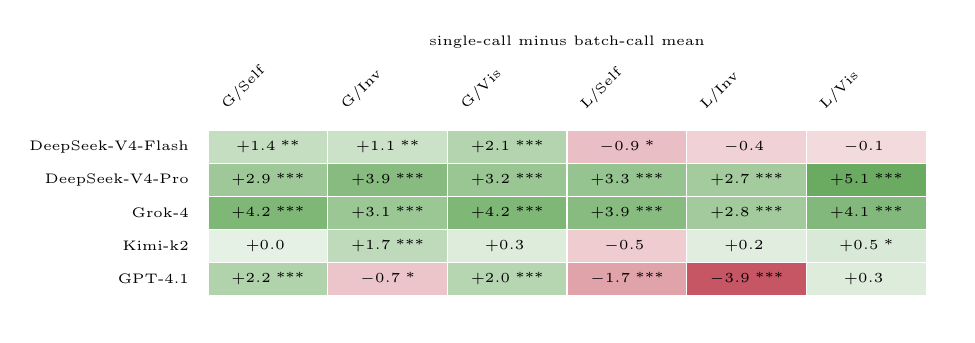
\begin{tikzpicture}[x=1cm,y=1cm,font=\tiny]
\path[use as bounding box] (0.05,1.10) rectangle (11.72,-2.55);
\node[font=\tiny] at (6.90,0.92) {single-call minus batch-call mean};
\node[rotate=45, anchor=west] at (2.46,0) {G/Self};
\node[rotate=45, anchor=west] at (3.98,0) {G/Inv};
\node[rotate=45, anchor=west] at (5.50,0) {G/Vis};
\node[rotate=45, anchor=west] at (7.02,0) {L/Self};
\node[rotate=45, anchor=west] at (8.54,0) {L/Inv};
\node[rotate=45, anchor=west] at (10.06,0) {L/Vis};
\node[anchor=east] at (2.22,-0.41) {DeepSeek-V4-Flash};
\filldraw[fill=grokc!35!white, draw=white] (2.34,-0.62) rectangle (3.86,-0.20);
\node at (3.10,-0.41) {$+1.4$\;**};
\filldraw[fill=grokc!31!white, draw=white] (3.86,-0.62) rectangle (5.38,-0.20);
\node at (4.62,-0.41) {$+1.1$\;**};
\filldraw[fill=grokc!46!white, draw=white] (5.38,-0.62) rectangle (6.90,-0.20);
\node at (6.14,-0.41) {$+2.1$\;***};
\filldraw[fill=riskred!28!white, draw=white] (6.90,-0.62) rectangle (8.42,-0.20);
\node at (7.66,-0.41) {$-0.9$\;*};
\filldraw[fill=riskred!20!white, draw=white] (8.42,-0.62) rectangle (9.94,-0.20);
\node at (9.18,-0.41) {$-0.4$\;};
\filldraw[fill=riskred!16!white, draw=white] (9.94,-0.62) rectangle (11.46,-0.20);
\node at (10.70,-0.41) {$-0.1$\;};
\node[anchor=east] at (2.22,-0.83) {DeepSeek-V4-Pro};
\filldraw[fill=grokc!58!white, draw=white] (2.34,-1.04) rectangle (3.86,-0.62);
\node at (3.10,-0.83) {$+2.9$\;***};
\filldraw[fill=grokc!72!white, draw=white] (3.86,-1.04) rectangle (5.38,-0.62);
\node at (4.62,-0.83) {$+3.9$\;***};
\filldraw[fill=grokc!61!white, draw=white] (5.38,-1.04) rectangle (6.90,-0.62);
\node at (6.14,-0.83) {$+3.2$\;***};
\filldraw[fill=grokc!63!white, draw=white] (6.90,-1.04) rectangle (8.42,-0.62);
\node at (7.66,-0.83) {$+3.3$\;***};
\filldraw[fill=grokc!55!white, draw=white] (8.42,-1.04) rectangle (9.94,-0.62);
\node at (9.18,-0.83) {$+2.7$\;***};
\filldraw[fill=grokc!90!white, draw=white] (9.94,-1.04) rectangle (11.46,-0.62);
\node at (10.70,-0.83) {$+5.1$\;***};
\node[anchor=east] at (2.22,-1.25) {Grok-4};
\filldraw[fill=grokc!77!white, draw=white] (2.34,-1.46) rectangle (3.86,-1.04);
\node at (3.10,-1.25) {$+4.2$\;***};
\filldraw[fill=grokc!60!white, draw=white] (3.86,-1.46) rectangle (5.38,-1.04);
\node at (4.62,-1.25) {$+3.1$\;***};
\filldraw[fill=grokc!77!white, draw=white] (5.38,-1.46) rectangle (6.90,-1.04);
\node at (6.14,-1.25) {$+4.2$\;***};
\filldraw[fill=grokc!72!white, draw=white] (6.90,-1.46) rectangle (8.42,-1.04);
\node at (7.66,-1.25) {$+3.9$\;***};
\filldraw[fill=grokc!56!white, draw=white] (8.42,-1.46) rectangle (9.94,-1.04);
\node at (9.18,-1.25) {$+2.8$\;***};
\filldraw[fill=grokc!75!white, draw=white] (9.94,-1.46) rectangle (11.46,-1.04);
\node at (10.70,-1.25) {$+4.1$\;***};
\node[anchor=east] at (2.22,-1.67) {Kimi-k2};
\filldraw[fill=grokc!15!white, draw=white] (2.34,-1.88) rectangle (3.86,-1.46);
\node at (3.10,-1.67) {$+0.0$\;};
\filldraw[fill=grokc!39!white, draw=white] (3.86,-1.88) rectangle (5.38,-1.46);
\node at (4.62,-1.67) {$+1.7$\;***};
\filldraw[fill=grokc!20!white, draw=white] (5.38,-1.88) rectangle (6.90,-1.46);
\node at (6.14,-1.67) {$+0.3$\;};
\filldraw[fill=riskred!22!white, draw=white] (6.90,-1.88) rectangle (8.42,-1.46);
\node at (7.66,-1.67) {$-0.5$\;};
\filldraw[fill=grokc!18!white, draw=white] (8.42,-1.88) rectangle (9.94,-1.46);
\node at (9.18,-1.67) {$+0.2$\;};
\filldraw[fill=grokc!23!white, draw=white] (9.94,-1.88) rectangle (11.46,-1.46);
\node at (10.70,-1.67) {$+0.5$\;*};
\node[anchor=east] at (2.22,-2.09) {GPT-4.1};
\filldraw[fill=grokc!47!white, draw=white] (2.34,-2.30) rectangle (3.86,-1.88);
\node at (3.10,-2.09) {$+2.2$\;***};
\filldraw[fill=riskred!25!white, draw=white] (3.86,-2.30) rectangle (5.38,-1.88);
\node at (4.62,-2.09) {$-0.7$\;*};
\filldraw[fill=grokc!44!white, draw=white] (5.38,-2.30) rectangle (6.90,-1.88);
\node at (6.14,-2.09) {$+2.0$\;***};
\filldraw[fill=riskred!40!white, draw=white] (6.90,-2.30) rectangle (8.42,-1.88);
\node at (7.66,-2.09) {$-1.7$\;***};
\filldraw[fill=riskred!73!white, draw=white] (8.42,-2.30) rectangle (9.94,-1.88);
\node at (9.18,-2.09) {$-3.9$\;***};
\filldraw[fill=grokc!20!white, draw=white] (9.94,-2.30) rectangle (11.46,-1.88);
\node at (10.70,-2.09) {$+0.3$\;};
\end{tikzpicture}
}}
    \captionof{figure}{序列效应Delta热力图（逐题独立调用减整卷作答）。}
    \label{fig:sequence_heatmap}
  \end{minipage}
\end{table*}


\FloatBarrier
